Space allocation of the subsystems described in the previous section, as well as crew members, is performed with the goals of:
\begin{itemize}
\item Accommodating subsystems necessary to support interplanetary flight and entry
\item Providing crew members with a habitable volume and operational items to support a flight duration of approximately 100 days
\item Keeping the axial position of the \gls{cg} forward to lower pitch stability and alleviate pitch control performance in the final mission phase
\item Allowing for packaging freedom in achieving a static lateral \gls{cg} offset for creating an asymmetric lifting shape
\end{itemize}
To this end, the crew module is packaged as depicted in Figures \ref{fig:axview}, \ref{fig:axview2} and \ref{fig:topview}. 

The top part is required to contain drogues to stabilise the entry vehicle in its final descent phase. Four drogues are placed to incorporate redundancy and provide a symmetric configuration, to prevent excessive tilting during final descent. Moreover, the top part contains the foldable solar arrays required to generate power required during interplanetary transfer. These are placed in the top part to prevent interference with firstly the exhaust flow from thrusters and secondly the stowed inflatable before entry on the other hand. A high-gain antenna of adjustable attitude on a boom enables communication during all mission phases. Thrusters for the apogee boost are mounted on top, of 0.41 $[m]$ length. Therefore the length of the top part is estimated on the basis hereof to be 0.50 $[m]$ length.

Crew members are located in the next part, a habitable volume to their availability that is dictated by the performance limit for a three-month mission duration as 11 $[m^{3}]$ per crew member \cite{Rudisill2008}. The diameter of the habitable volume is 4.0 $[m]$, thereby less than vehicle maximum diameter to accommodate four propellant tanks, one per quadrant. Propellant tanks allow intertank propellant transfer to maintain the lateral \gls{cg} position. The tanks are sized on the basis of the total required propellant and provide propellant for both the reaction control thrusters, apogee boosters and retro-propulsion thruster assembly. The length of this part follows from the habitable volume and depends on the number of crew members. For two crew members, it is 1.75 $[m]$ long. Including a 0.25 $[m]$ contingency for an aft pressure bulkhead yields an estimated length of 2.00 $[m]$.

Operational items are located within reach of crew members. These are placed at this location because of their relatively high mass and therefore contribution to the axial \gls{cg} position. The total volume occupied follows from Table \ref{tab:crewmemberops}. On one hand these operational items include relatively dense products, foremostly the life support systems, and less dense products in the form of food and other supplies.  The length of this part follows from the required volume for operational items, for two crew members equal to 0.75 $[m]$. Including a forward additional bulkhead yields an estimated length of 1.00 $[m]$.

%Arranging these items asymmetrically allows for a lateral \gls{cg} offset, most notably considering the depleted supplies of food at the end of interplanetary transfer while life support system mass remains intact.

Four struts for touchdown, packed symmetrically. The struts are arranged about the batteries required to provide power during entry, when solar panels are stowed, and the main thrusters for retro-propulsion. The length follows from estimates for the strut required volume and the retro-propulsion thrusters of 2.30 $[m]$ length. It is an estimated 2.0 $[m]$, as part of the thruster is contained within the last part.

The last part contains the thruster nozzle, closed off by a heat-resistant end-cap during entry, a nitrogen tank and inflation system, and the attachment rings for the inflatable decelerator. The end-cap is to be eject-able. The length of this part is mainly dictated by the shape of the inflatable and where it attaches to the centre body. For a 12.0 $[m]$ deployed diameter, it is approximately 1.0 [$m$] in length.

This yields a total vehicle length of an estimated 6.5 $[m]$. This fits within \gls{sls} fairing constraints  and moreover ensures that the crew module is not impinged by the flow.

\begin{figure}[ht]
		\centering
		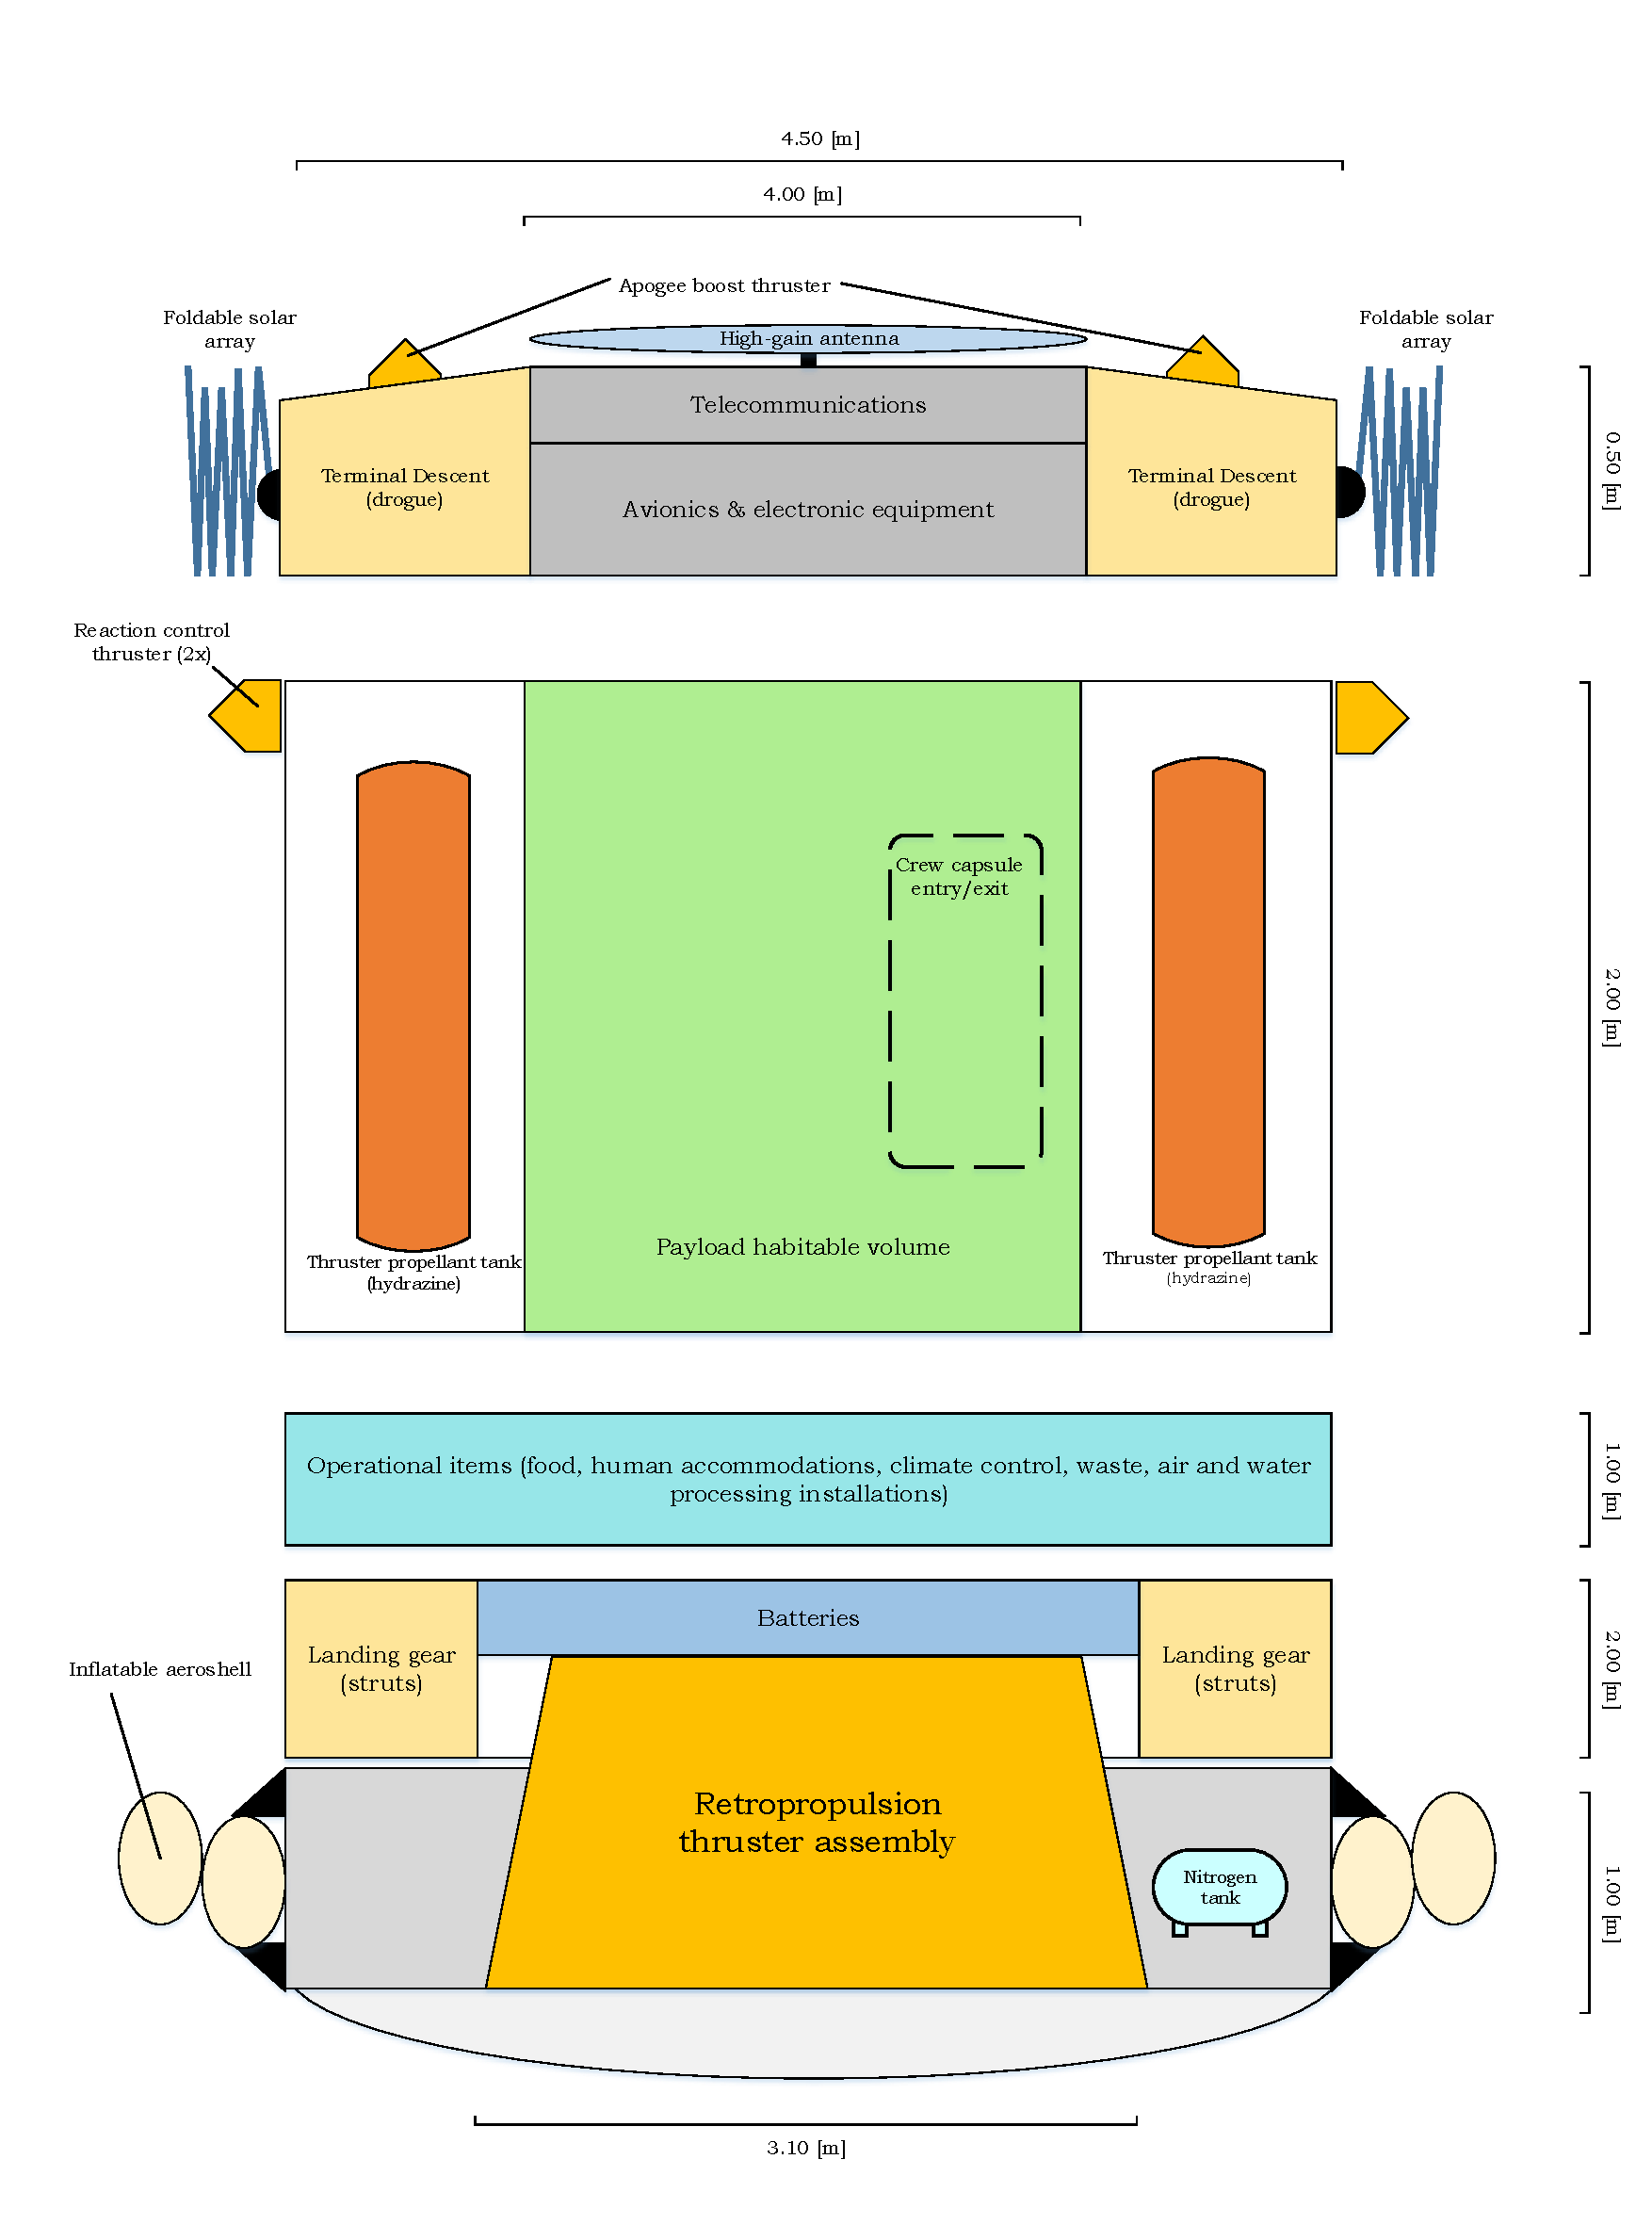
\includegraphics[width=0.95\textwidth]{./Figure/CrewModule/Axialview.pdf}
		\caption[First axial view of crew module lay-out]{First axial view of crew module lay-out. Drawing not to scale.}
		\label{fig:axview}
\end{figure}

\begin{figure}[ht]
		\centering
		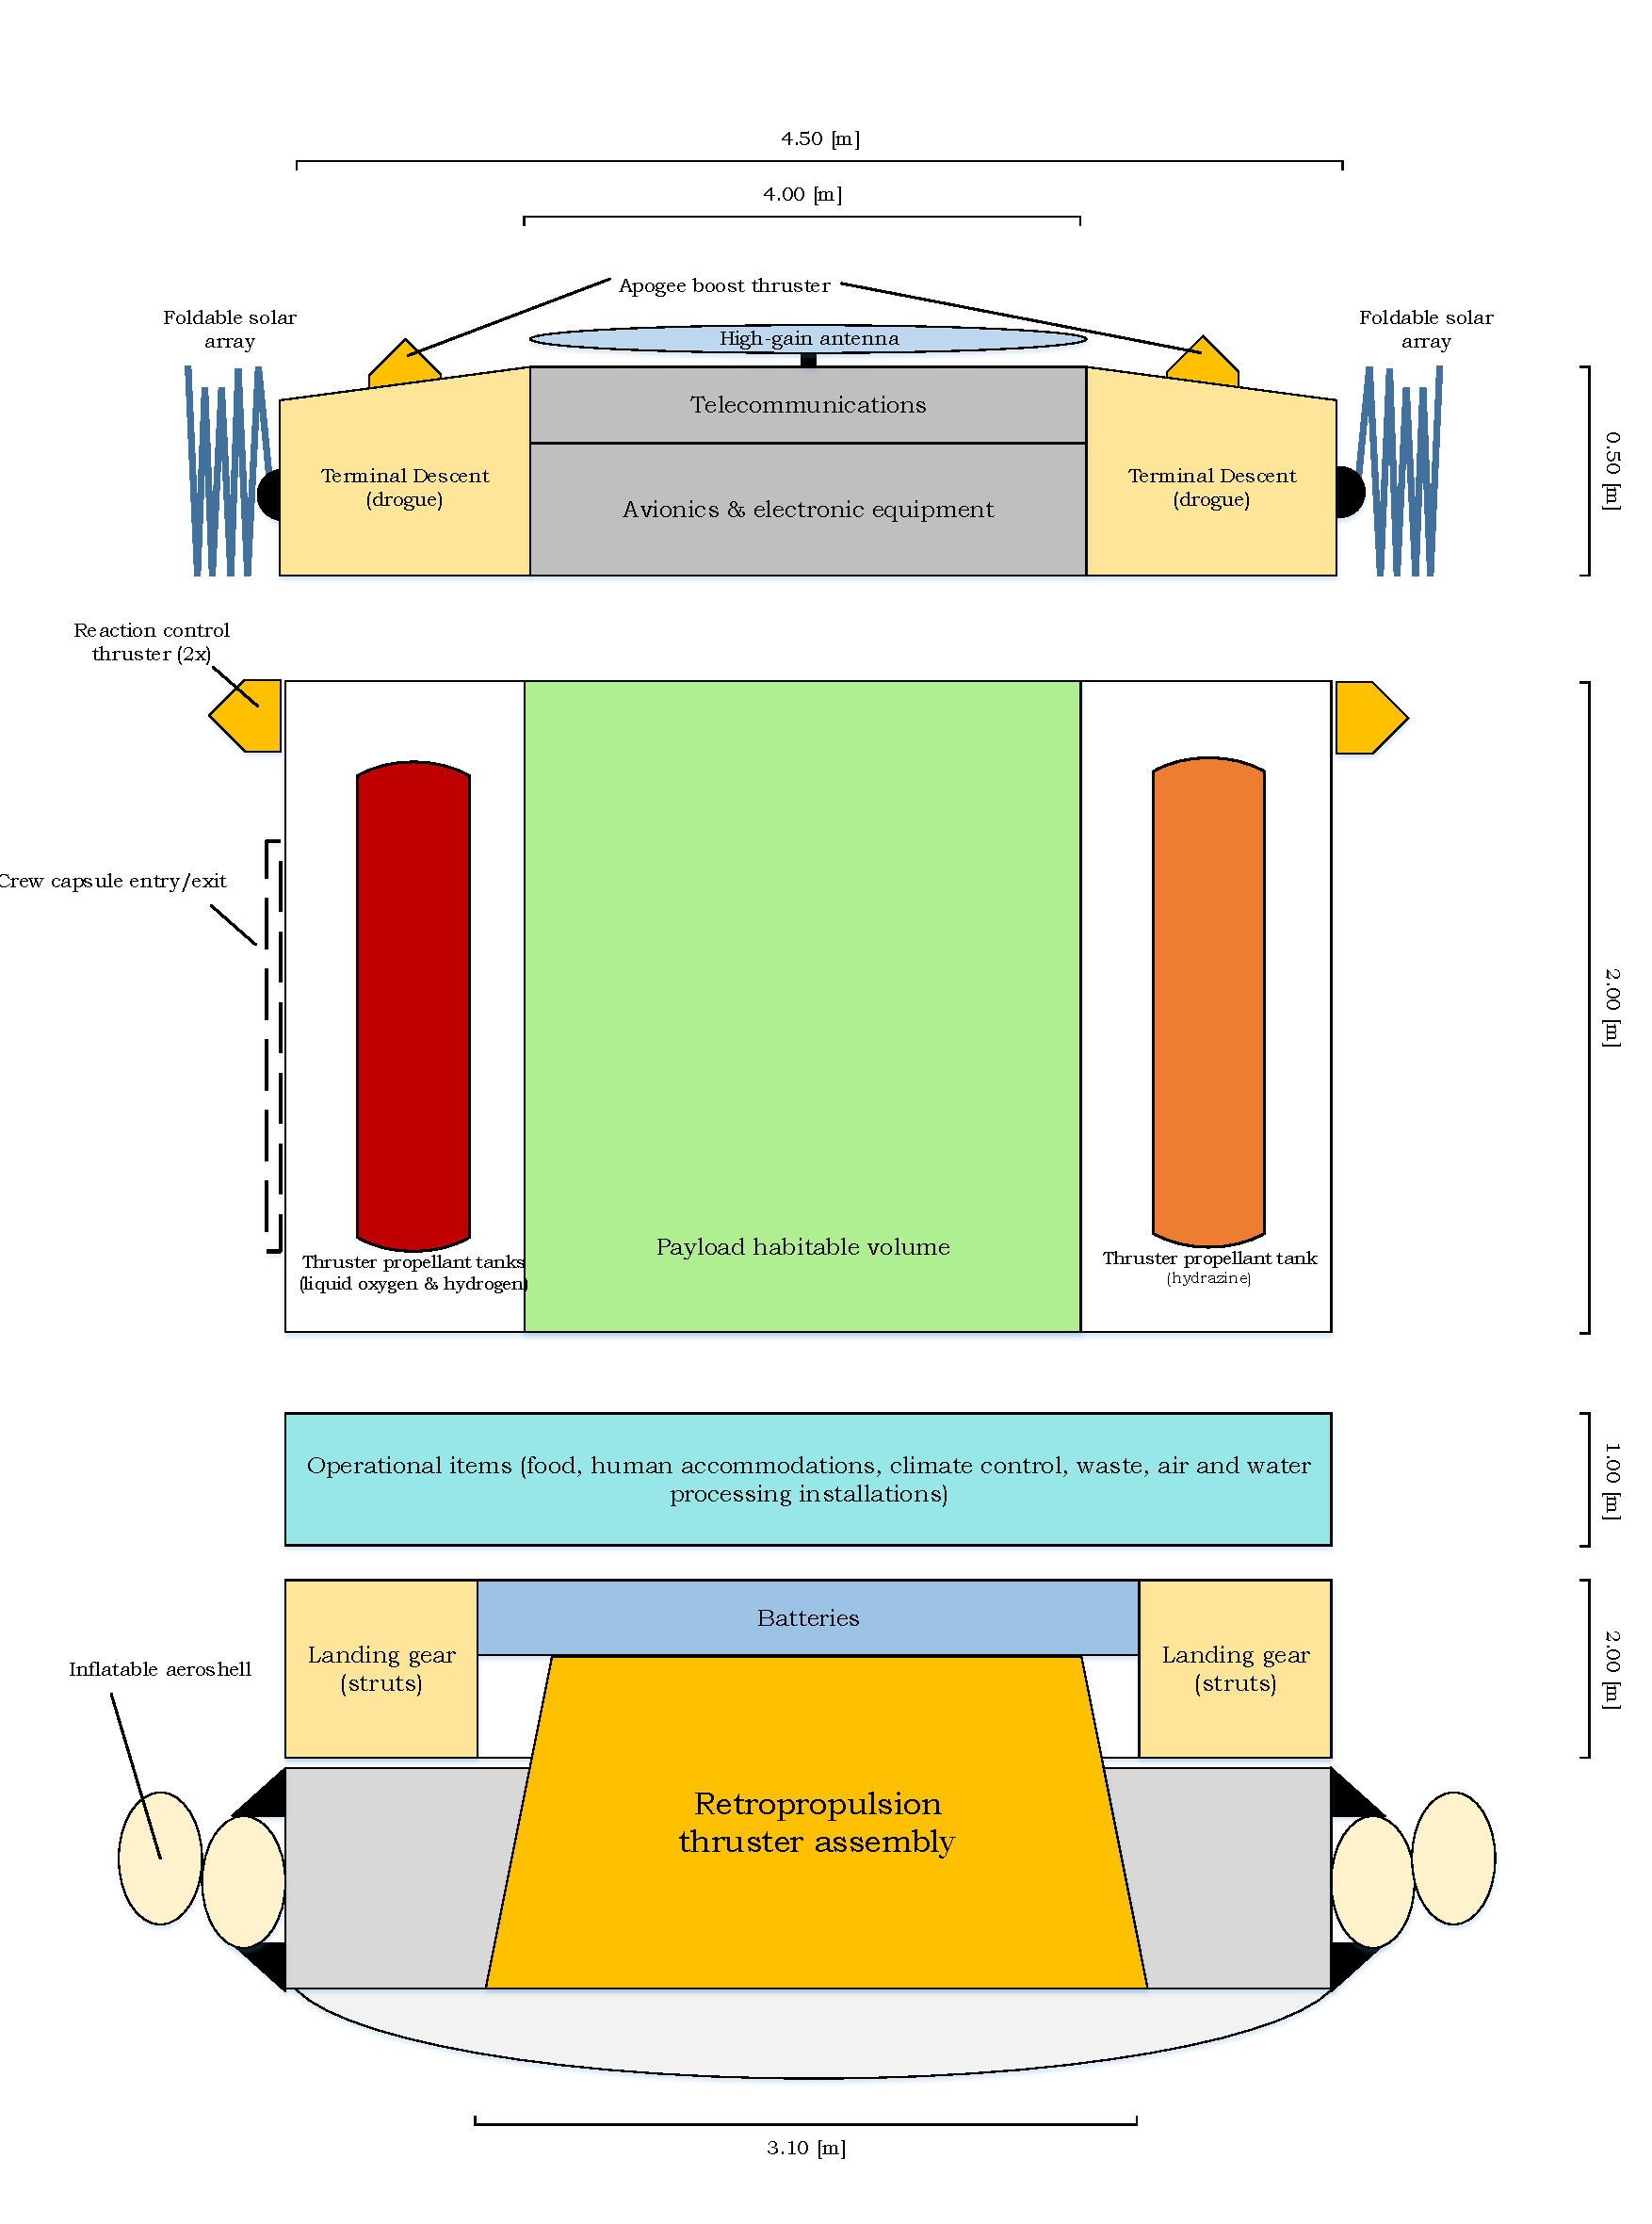
\includegraphics[width=0.95\textwidth]{./Figure/CrewModule/Axialview2.pdf}
		\caption[Second axial view of crew module lay-out]{Second axial view of crew module lay-out. Drawing not to scale.}
		\label{fig:axview2}
\end{figure}

\begin{figure}[ht]
		\centering
		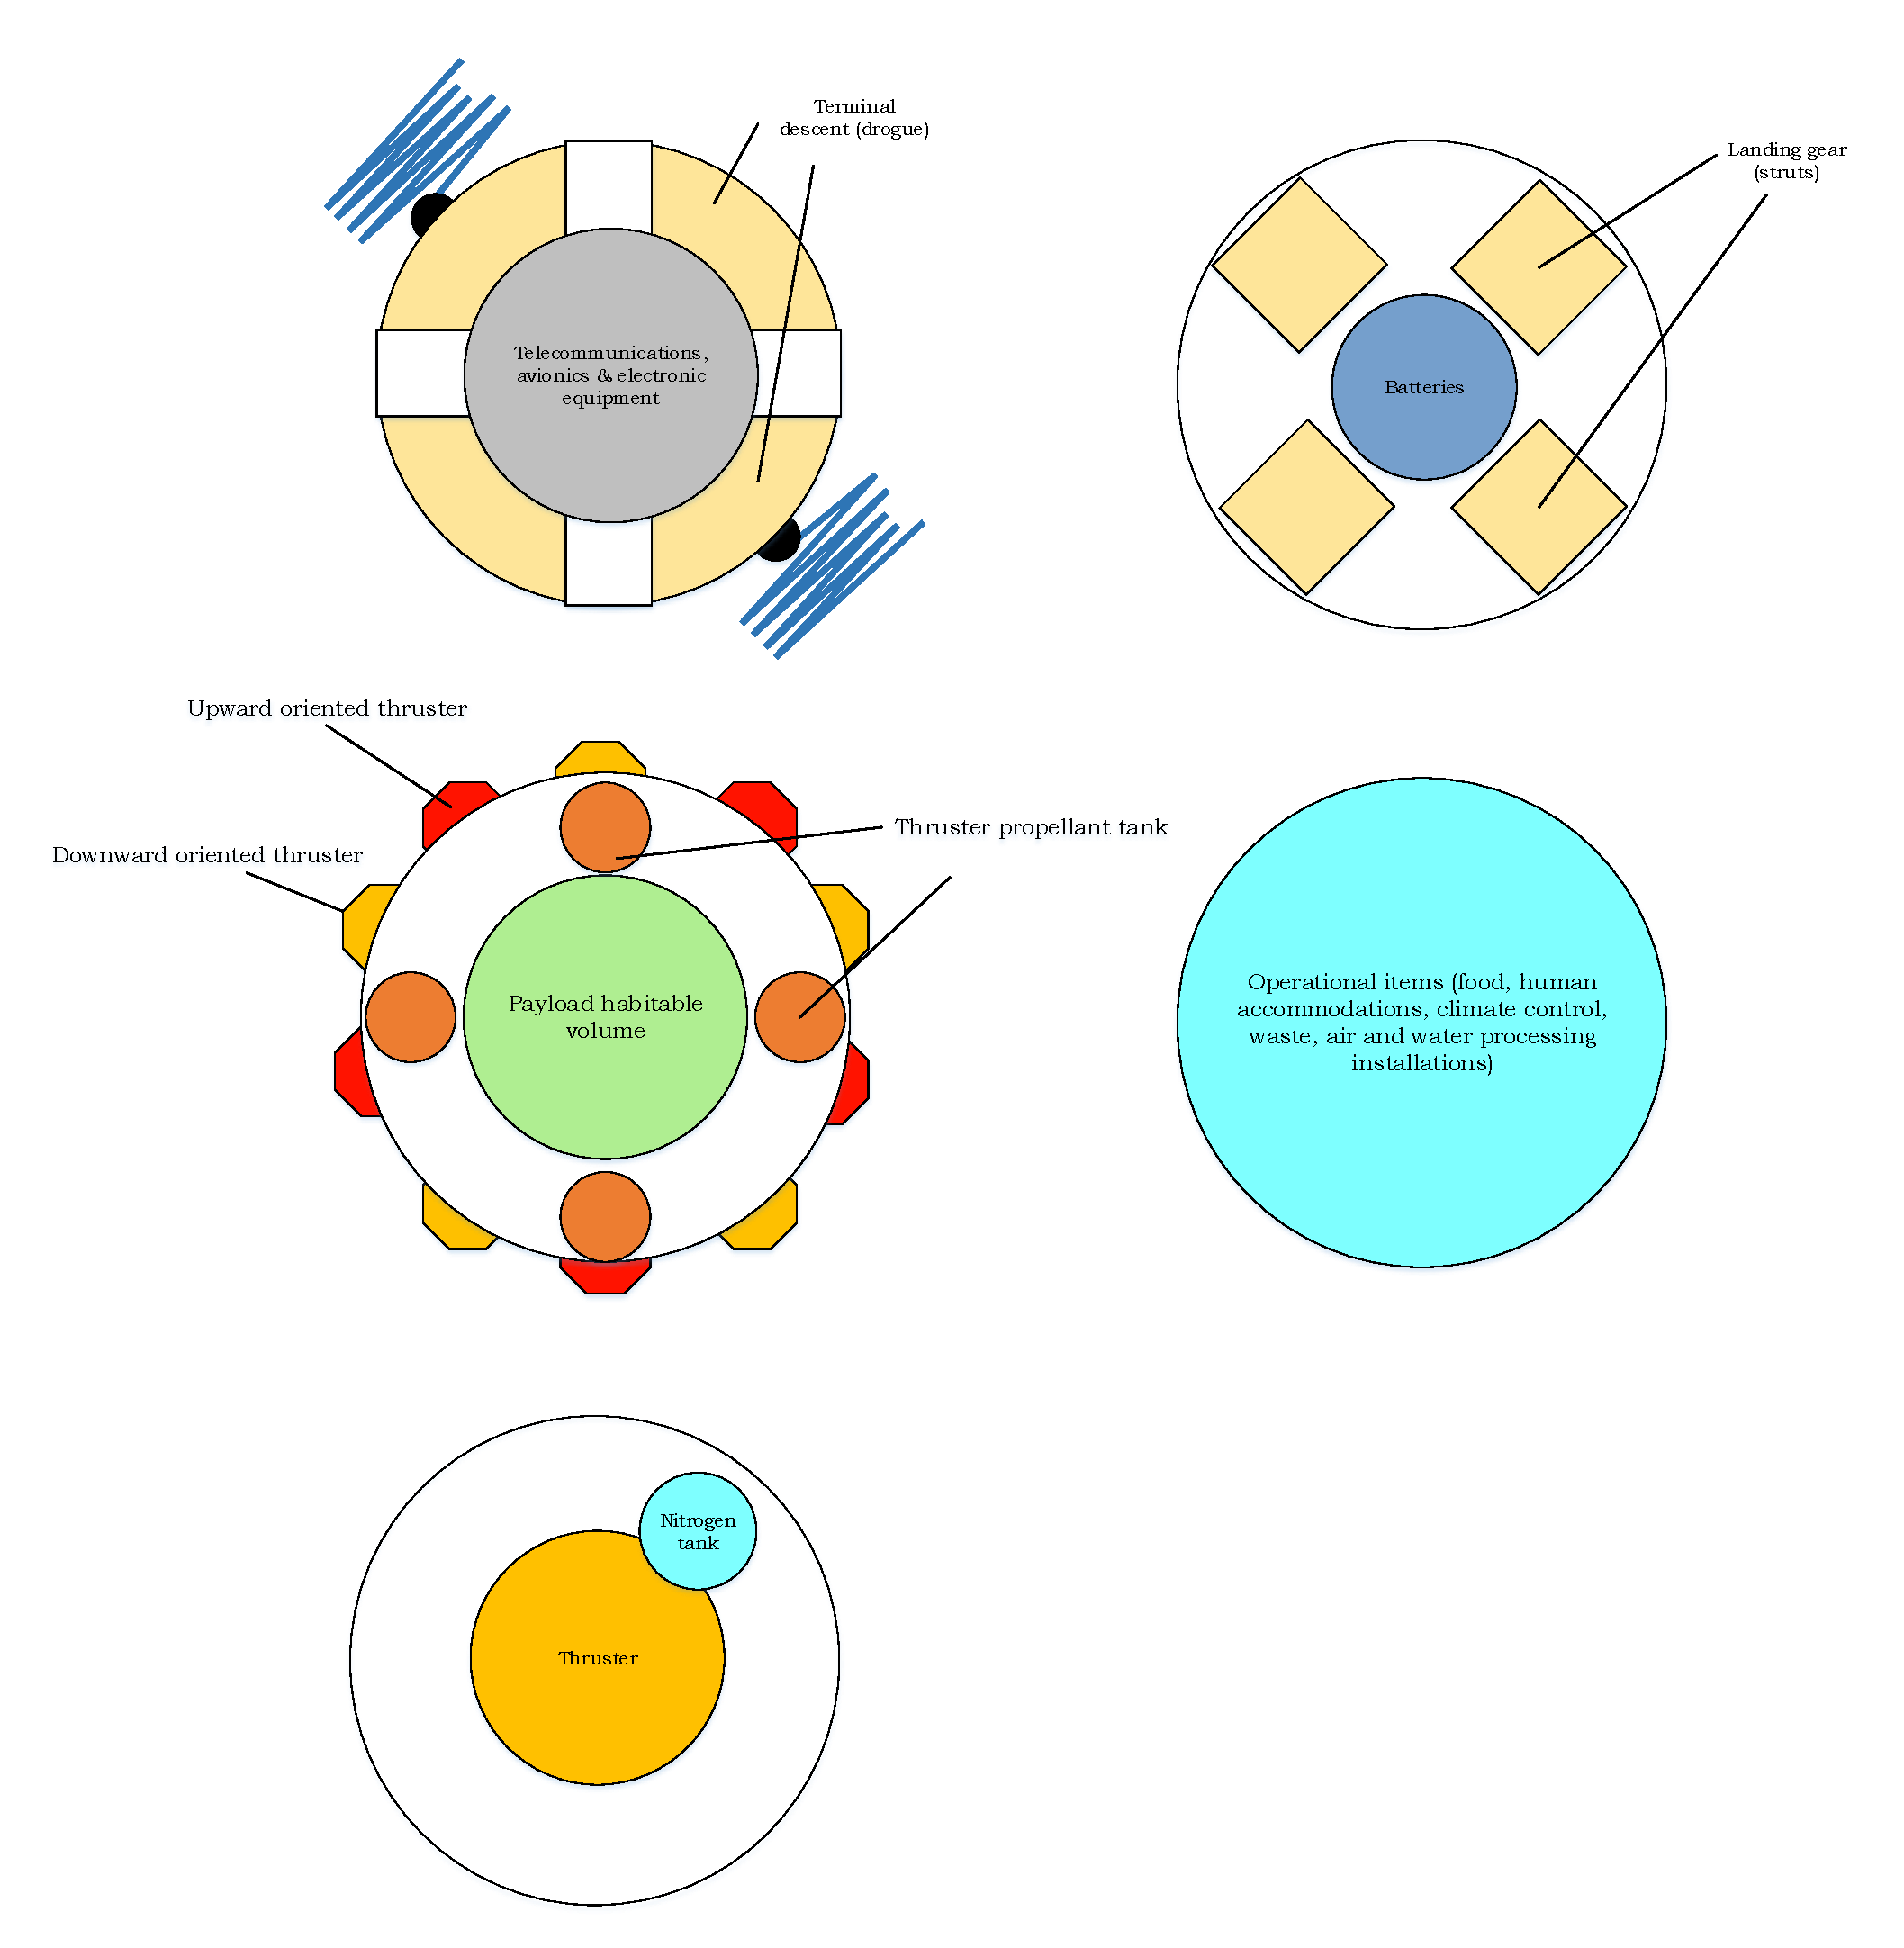
\includegraphics[width=0.95\textwidth]{./Figure/CrewModule/TopviewV2.pdf}
		\caption[Top-down view of crew module lay-out]{Top-down view of crew module lay-out. Drawing not to scale.}
		\label{fig:topview}
\end{figure}

Component masses are as listed in Table \ref{tab:crewmass}. Due to the relative large weight of items closer to the aeroshell the axial \gls{cg} position is estimated closer than 3 $[m]$ from the inflatable aeroshell attachment point. A more elaborate estimate is without value, for the actual packaging of the crew module requires a more thorough design beyond the mission scope. However, to investigate the feasibility of achieving the required \gls{cg} offset, it follows from Figure \ref{fig:cgoffset} that the required \gls{cg} offset is below 0.5 $[m]$. Such an offset can be affected primarily by shifting the relatively heavy contributions of operational items. Placing the \gls{cg} thereof 1.5 $[m]$ from the axial centreline and assuming a symmetric configuration otherwise yields an approximate 0.5 $[m]$ lateral \gls{cg} offset. Considering the 4.5 $[m]$ diameter allocated to operational items, this is feasible. %In addition, pumping fuel from tank to tank provides a measure of \gls{cg} position control.

\begin{table}[ht]
\centering
\caption{Crew module mass budget}
\label{tab:crewmass}
\begin{tabular}{|l|c|}
\hline
{\bf Component}    & {\bf Component mass {[}kg{]}} \\ \hline \hline
Power              & 280                           \\ \hline
 ADCS        &  225                     \\ \hline
Thermal            & 600                           \\ \hline
Structural mass    & 1300                          \\ \hline
Operational items  & 3140                          \\ \hline
Crew               & 160                           \\ \hline
Terminal descent   & 1445                          \\ \hline
C\&DH              & 585                           \\ \hline 
Other    & 815                          \\ \hline \hline
\textbf{Total}    & \textbf{8 550}                          \\ \hline \hline
Margin ($5\%$)  & 450                        \\ \hline \hline
{\bf Capsule mass} & {\bf 9 000}                    \\ \hline
\end{tabular}
\end{table}


